\documentclass{beamer}
\usepackage[utf8]{inputenc}
\usepackage[T1]{fontenc}
\usepackage[english,french]{babel}
\usepackage{tabularx}
\usepackage{graphicx}
\usepackage{epstopdf}
\usepackage{pifont}

\usetheme{Antibes}
\title[CryptoSMS]{CryptoSMS\\Text message encryption for Android}
\author{David Brazdil}
\institute{University of Cambridge}
\date{September 15, 2011}

% getting rid of sections and subsections
\setbeamertemplate{headline} {
\begin{beamercolorbox}{section in head/foot}
	\vskip2pt
	\vskip10pt
\end{beamercolorbox}
}
\setbeamertemplate{navigation symbols}{} 

% tick and fail commands
\newcommand*\tick{\item[\ding{51}]}
\newcommand*\fail{\item[\ding{55}]}

% TEXT CONSTANTS
\newcommand{\txtTextCompression}{Text compresses very well}

% MARGIN AND PADDING IN TABLES
\renewcommand*\arraystretch{1.5}
\newcommand{\verticalspace}{\vspace{10pt}}

\begin{document}
\newcolumntype{L}{>{\raggedright\arraybackslash}X}%

\begin{frame}
	\titlepage
\end{frame}

% FACTS

\begin{frame}{Powerful enemies}
	\begin{itemize}
		\item{Can read and manipulate everything you send}
		\item{Can send a message from arbitrary phone number}
		\item{Can gain physical access to your handset}
		\item{Can install a malicious application on your phone}
	\end{itemize}
\end{frame}

\begin{frame}{Strong protection}
	\vfill
	\begin{itemize}
		\item{Messages encrypted with AES-256/CBC/HMAC-SHA-256}
		\item{Key negotiation with Elliptic Curve Diffie-Hellman}
		\item{Authentication provided by external application}
		\item{Forward secrecy}
		\item{All data stored in an encrypted file}
	\end{itemize}
	\vfill
	\begin{flushright}
	\emph{With thanks to Richard Clayton and Joseph Bonneau}
	\end{flushright}
\end{frame}

% DEMO

% TEXT MESSAGING

\begin{frame}{Data SMS standard}
	\begin{itemize}
		\item{sent to a specific port}
		\item{not stored by the OS}
		\item{133 bytes instead of 140}
		\item{long messages divided into multiple parts}
		\begin{itemize}
			\item{84 bytes in first part}
			\item{130 bytes in other parts}
		\end{itemize}
		\item{text compression with DEFLATE}
	\end{itemize}
\end{frame}

%\begin{frame}{Message structure}
%	\begin{block}{First part}
%		\verticalspace
%		\begin{tabularx}{\textwidth}{ |l|l|l|l|L| }
%			\hline
%			mt1, count  & ID      & IV   & MAC & data \\
%			1 B         & 2 B     & 16 B & 32 B & 84 B  \\
%			\hline
%		\end{tabularx}
%	\end{block}
%
%	\begin{block}{Other parts}
%		\verticalspace
%		\begin{tabularx}{\textwidth}{ |l|l|L| }
%			\hline
%			mt2, index  & ID   & data \\
%			1 B         & 2 B     & 130 B  \\
%			\hline
%		\end{tabularx}
%	\end{block}
%	
%	\begin{itemize}
%		\item{mt1, mt2 - message types}
%	\end{itemize}
%\end{frame}

\begin{frame}{\txtTextCompression}
	\begin{exampleblock}{French}
		\foreignlanguage{french}{Salut Pierre, {\c c}a va? Je suis désolé, mais je ne serai pas là à cinq heures, parce que je suis malade. Je suis libre ce lundi et toi? Quand tu as quelques problèmes, appelles-moi. J'espère que tout sera ok.}

		\verticalspace
		\centering
		\begin{tabular}{ |c|c|c|c| }
			\hline
			UTF-16 & UTF-16 + DEFLATE & UTF-8 & UTF-8 + DEFLATE \\
			\hline
			412 B & 210 B & 212 B & 164 B \\
			\hline
		\end{tabular}
	\end{exampleblock}
\end{frame}

\begin{frame}{\txtTextCompression}
	\begin{exampleblock}{Hebrew}
		\begin{flushright}
			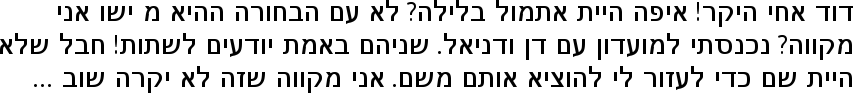
\includegraphics[width=\textwidth]{hebrew}
		\end{flushright}
		\centering
		\begin{tabular}{ |c|c|c|c| }
			\hline
			UTF-16 & UTF-16 + DEFLATE & UTF-8 & UTF-8 + DEFLATE \\
			\hline
			404 B & 201 B & 353 B & 189 B \\
			\hline
		\end{tabular}
	\end{exampleblock}
\end{frame}


% KEY NEGOTIATION

%\begin{frame}{Elliptic Curve Deffie-Hellman}
%	\begin{block}{Alice $\rightarrow$ Bob}
%		\[
%			mt3, t1, DH_A, \{ h( mt3, t1, DH_A ) \}_{P^{-1}_A}
%		\]
% 	\end{block}
%	\begin{block}{Bob $\rightarrow$ Alice}
%		\[
%			mt4, t2, DH_B, \{ h( mt3, t1, DH_A, mt4, t2, DH_B ) \}_{P^{-1}_B}
%		\]
% 	\end{block}
%
%	\begin{itemize}
%		\item{t1, t2 - timestamps}
%		\item{$DH_A$, $DH_B$ - Deffie-Hellman public keys}
%	\end{itemize}
%\end{frame}

% STORAGE FILE

\begin{frame}{Storage file}
	\begin{itemize}
		\item{stores all data encrypted}
		\item{does not reveal its internal structure}
		\item{not necessary to decrypt the whole file}
		\item{speed optimized for the most common tasks}
	\end{itemize}
\end{frame}

\begin{frame}{Storage file structure}
	\centering
	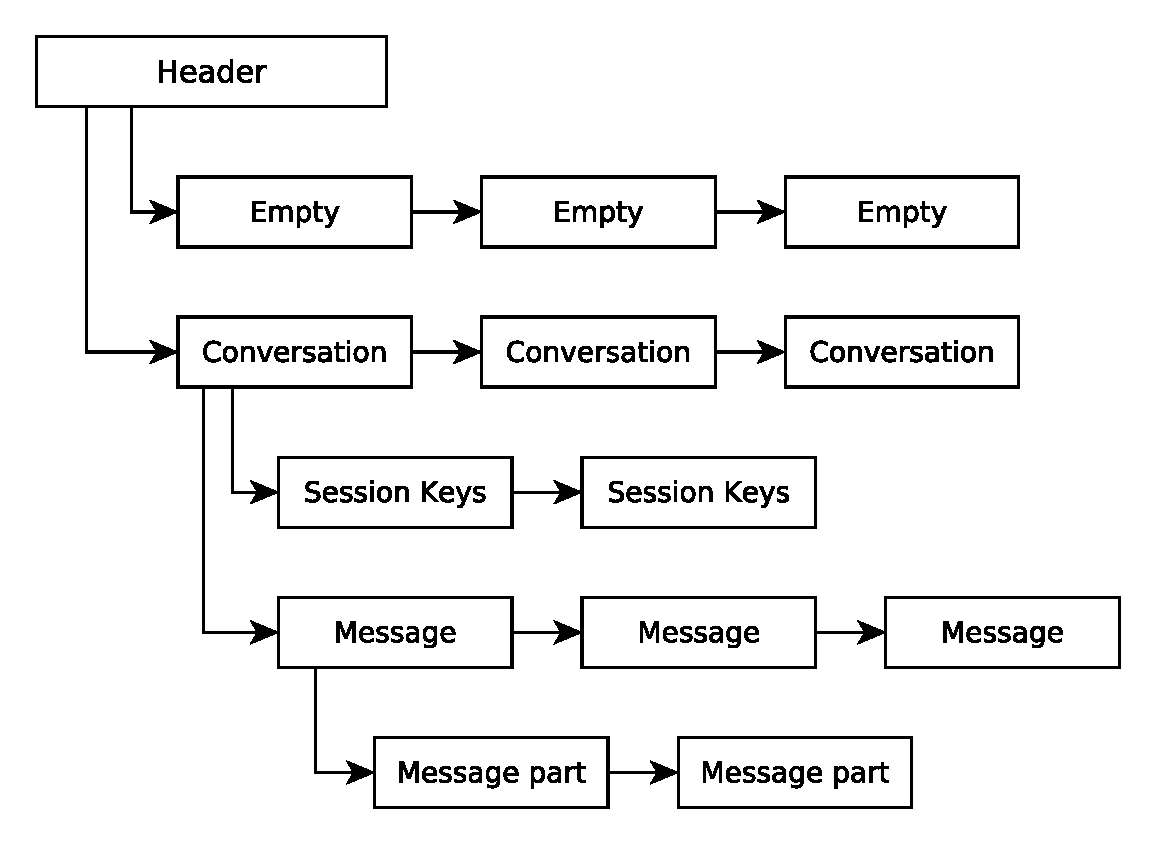
\includegraphics[width=0.8\textwidth]{storage_file}
\end{frame}

\begin{frame}{Reveals nothing to the outside}
	\begin{tabularx}{\textwidth}{ |l|l|L| }
		\hline
		IV & MAC & Encrypted header \\
		\hline
		IV & MAC & Encrypted entry 1 \\
		\hline
		IV & MAC & Encrypted entry 2 \\
		\hline
		IV & MAC & Encrypted entry 3 \\
		\hline
		IV & MAC & Encrypted entry 4 \\
		\hline
		IV & MAC & Encrypted entry 5 \\
		\hline
		IV & MAC & Encrypted entry 6 \\
		\hline
		IV & MAC & Encrypted entry 7 \\
		\hline
	\end{tabularx}

	\centering
	$\vdots$ \\
\end{frame}

% PKI COOPERATION

\begin{frame}{Cooperation with the Key Ring}
	\begin{itemize}
		\item{Signs data and verifies signatures}
		\item{Shared login session}
		\item{Application locks itself after logging out}
		\item{Storage file key stored in the Key Ring}
	\end{itemize}
\end{frame}

% SUMMARY

\begin{frame}{Achievements and issues}
	\begin{itemize}
		\fail Uninstalling the Key Ring deletes the storage key
		\tick Messages encrypted and authenticated
		\tick Data protected in a safe storage file
 	\end{itemize}
\end{frame}

\end{document}